\section{IP Addresses of Interfaces}
\label{sec:IP}

% \subsection{Design}

Assigning IP addresses to interfaces should be the first step in building BT Network since all network services listed in \ref{sec:services} cannot operate without IP addresses.
The assignment of IP addresses in Table \ref{tab:ip} and \ref{tab:interfaces} is implemented.

\subsection{Implementation}

\subsubsection{Routers}

For Router 1 (BT-R001), IP addresses are assigned directly to physical interfaces as all interfaces are network layer interfaces.

\begin{lstlisting}
int fa0/0
ip address 23.0.0.49 255.255.255.252
ipv6 address 2001:2300:0:3::1/64
no shutdown

int fa0/1
ip address 23.0.0.57 255.255.255.252
ipv6 address 2001:2300:0:5::1/64
no shutdown

int fa0/1/0
ip address 23.0.0.1 255.255.255.240
ipv6 address 2001:2300:0:0::1/64
no shutdown
\end{lstlisting}

For Router 2 (BT-R002), however, only $2$ interfaces (\texttt{FastEhternet0/0} and \texttt{FastEhternet0/1}) each are network layer interfaces. The remaining $4$ interfaces are link layer interfaces and need to be assigned to an VLAN separately se where an IP address can be assigned. 

\begin{lstlisting}
int fa0/0
ip address 23.0.0.50 255.255.255.252
ipv6 address 2001:2300:0:3::2/64
no shutdown

int fa0/1
ip address 23.0.0.53 255.255.255.252
ipv6 address 2001:2300:0:4::1/64
no shutdown

vlan 1
int fa0/1/0
switchport mode access
switchport access vlan 1
int vlan 1
ip address 23.0.0.17 255.255.255.240
ipv6 address 2001:2300:0:1::1/64
no shutdown

vlan 3
int fa0/1/1
switchport mode access
switchport access vlan 3
int vlan 3
ip address 23.0.0.61 255.255.255.252
ipv6 address 2001:2300:0:6::1/64
no shutdown
\end{lstlisting}

Similarly, IP addresses are assigned to Router 3 (BT-R003).

\begin{lstlisting}
int fa0/0
ip address 23.0.0.58 255.255.255.252
ipv6 address 2001:2300:0:5::2/64
no shutdown

int fa0/1
ip address 23.0.0.54 255.255.255.252
ipv6 address 2001:2300:4::2/64
no shutdown

vlan 2
int fa0/1/0
switchport mode access
switchport access vlan 2
int vlan 2
ip address 23.0.0.33 255.255.255.240
ipv6 address 2001:2300:0:2::1/64
no shutdown

vlan 4
int fa0/1/2
switchport mode access
switchport access vlan 4
int vlan 4
ip address 56.0.0.62 255.255.255.252
ipv6 address 2001:5600:0:6::2/64
no shutdown

vlan 5
int fa0/1/1
switchport mode access
switchport access vlan 5
int vlan 5
ip address 100.100.2.2 255.255.255.252
no shutdown
\end{lstlisting}

\subsubsection{Laptops}

Unlike routers, the IP assignment of laptops' interfaces are more aligned since all laptops are of the same model. 
On Laptop 1 (BT001), the file \texttt{/etc/network/interface} is edited as follows before rebooting to apply changes. 
Similarly, IP address can are assigned to Laptop 2's (BT002) and Laptop 3's interfaces respectively.

\begin{lstlisting}[language=sh]
auto lo
iface lo inet loopback
auto eth0
ifacce eth0 inet static 
address 23.0.0.2
netmask 255.255.255.240
gateway 23.0.0.1

ifacce eth0 inet6 static 
address 2001:2300::2
netmask 64
gateway 2001:2300::1
\end{lstlisting}

\subsection{Evaluation}

On all $3$ routers, the implementation of IP assignments is evaluated using \texttt{show ip int brief} and \texttt{show ipv6 int brief}. These $2$ commands show IPv4 and IPv6 addresses of interfaces on routers respectively.
Sucessful assignment of IP addresses to routers' interfaces is evident from Figure \ref{fig:ipv4-router} and \ref{fig:ipv6-router}.

\begin{figure*}[ht!]
    \centering
    \begin{subfigure}[b]{0.67\textwidth}
        \centering
        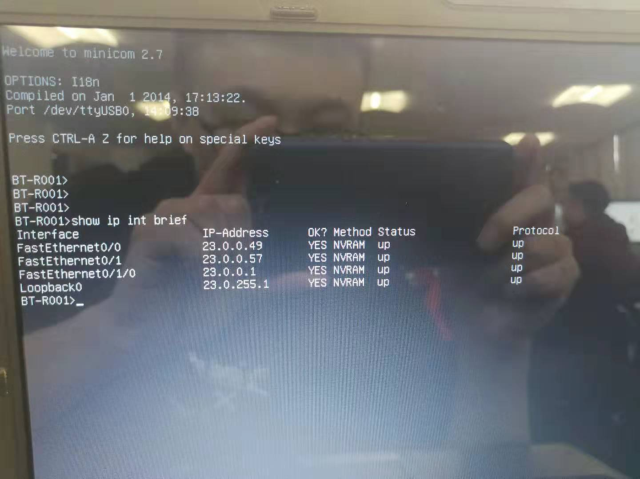
\includegraphics[width=\linewidth]{ipv4-router1}
        \caption{Router 1 (BT-R001)}
    \end{subfigure}
    \hfill
    \begin{minipage}[b]{0.3\textwidth}
	    \begin{subfigure}[b]{\linewidth}
	        \centering
	        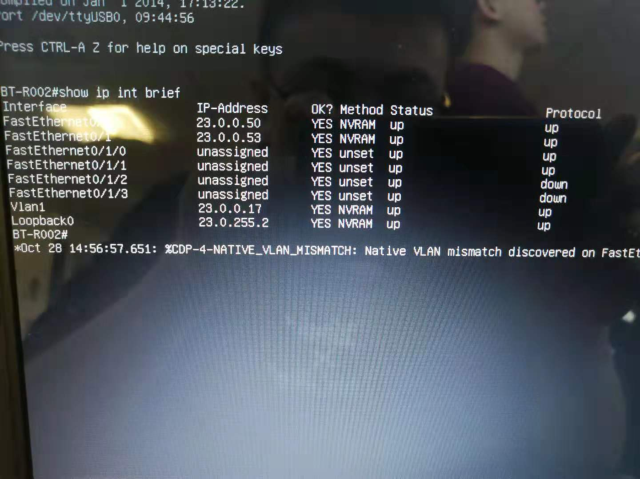
\includegraphics[width=\linewidth]{ipv4-router2}
	        \caption{Router 2 (BT-R002)}
	    \end{subfigure}
	    \\
	    \begin{subfigure}[b]{\linewidth}
	        \centering
	        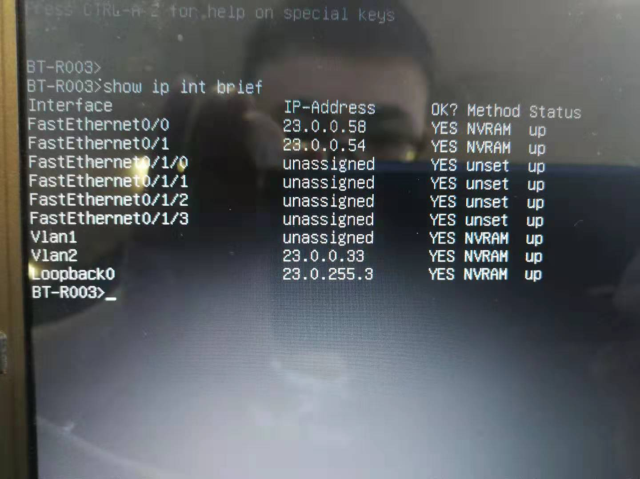
\includegraphics[width=\linewidth]{ipv4-router3}
	        \caption{Router 3 (BT-R003)}
	    \end{subfigure}
	\end{minipage}
    \caption{Sucessful Assignment of IPv4 Addresses to Routers' Interfaces.}
    \label{fig:ipv4-router}
\end{figure*}

\begin{figure*}[ht!]
    \centering
    \begin{subfigure}[b]{0.67\textwidth}
        \centering
        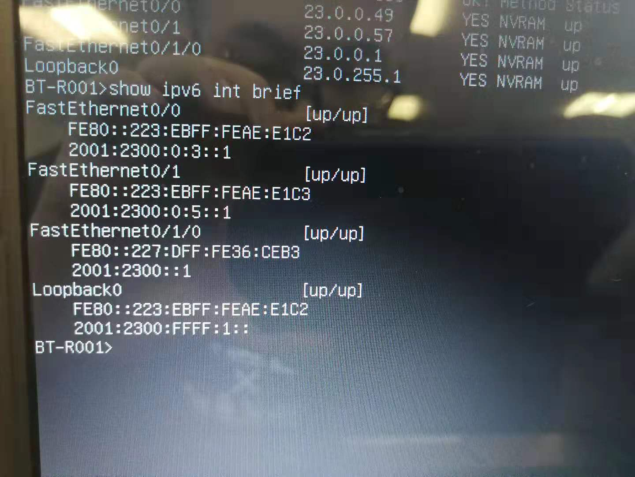
\includegraphics[width=\linewidth]{ipv6-router1}
        \caption{Router 1 (BT-R001)}
    \end{subfigure}
    \hfill
    \begin{minipage}[b]{0.3\textwidth}
	    \begin{subfigure}[b]{\linewidth}
	        \centering
	        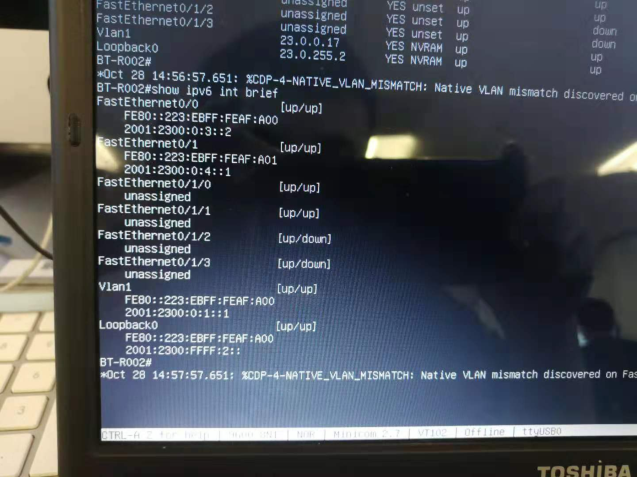
\includegraphics[width=\linewidth]{ipv6-router2}
	        \caption{Router 2 (BT-R002)}
	    \end{subfigure}
	    \\
	    \begin{subfigure}[b]{\linewidth}
	        \centering
	        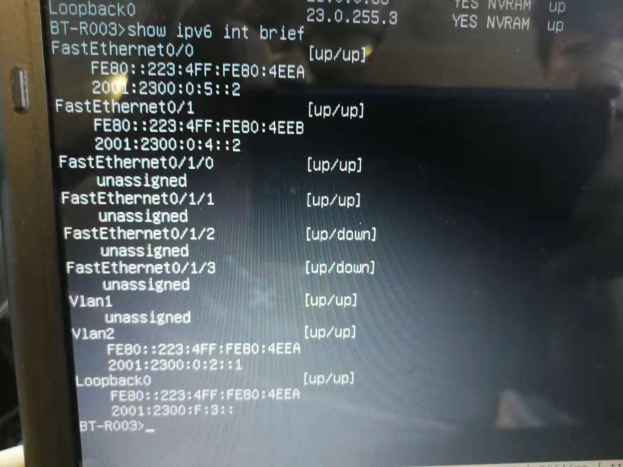
\includegraphics[width=\linewidth]{ipv6-router3}
	        \caption{Router 3 (BT-R003)}
	    \end{subfigure}
	\end{minipage}
    \caption{Sucessful Assignment of IPv6 Addresses to Routers' Interfaces.}
    \label{fig:ipv6-router}
\end{figure*}


On the laptops' side, the implementation of IP assignments is evaluated using \texttt{ifconfig} command.
Sucessful assignment of IP addresses to laptops' interfaces is evident from Figure \ref{fig:ip-laptop}.

\begin{figure*}[ht!]
    \centering
    \begin{subfigure}[b]{0.67\textwidth}
        \centering
        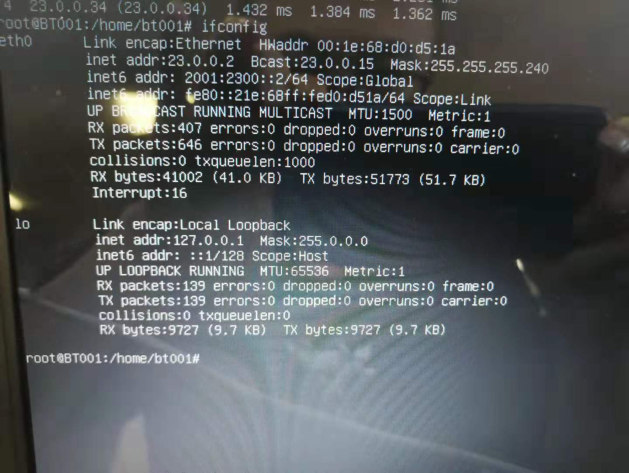
\includegraphics[width=\linewidth]{ip-laptop1}
        \caption{Laptop 1 (BT001)}
    \end{subfigure}
    \hfill
    \begin{minipage}[b]{0.3\textwidth}
	    \begin{subfigure}[b]{\linewidth}
	        \centering
	        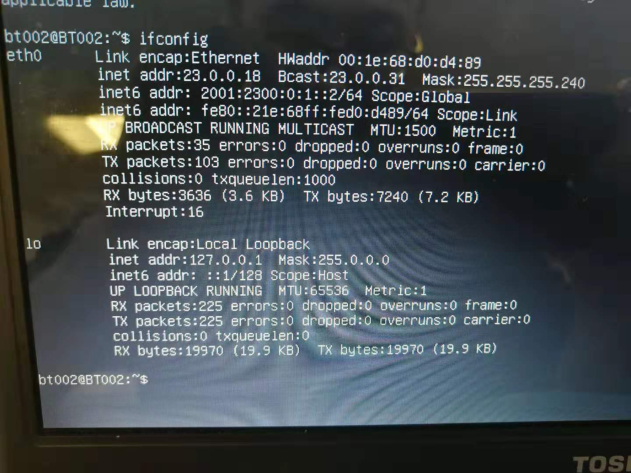
\includegraphics[width=\linewidth]{ip-laptop2}
	        \caption{Laptop 2 (BT002)}
	    \end{subfigure}
	    \\
	    \begin{subfigure}[b]{\linewidth}
	        \centering
	        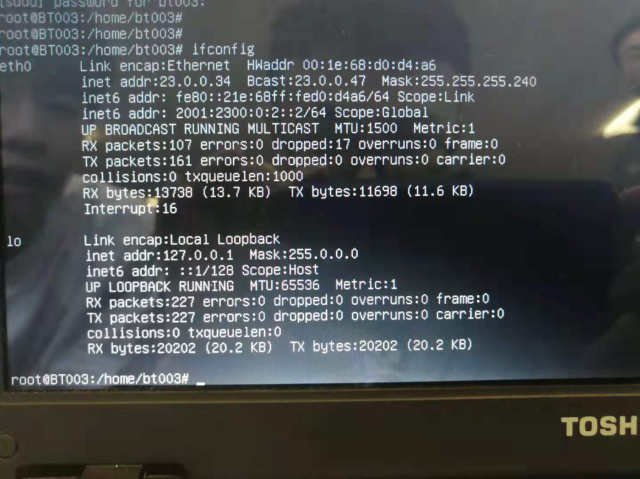
\includegraphics[width=\linewidth]{ip-laptop3}
	        \caption{Laptop 3 (BT003)}
	    \end{subfigure}
	\end{minipage}
    \caption{Sucessful Assignment of IPv4 and IPv6 Addresses to Laptops' Interfaces.}
    \label{fig:ip-laptop}
\end{figure*}

% \subsection{Commentary}

